\section{Methodology}

The section methodology describes the techniques, software, and datasets used to realize the project. Furthermore, the author gives insight into concrete implementation details.

\subsection{Technologies}

The development of a GAN is possible with various technologies. This section briefly introduces the core technologies of the project.

\subsubsection{PyTorch}

PyTorch\footnote{PyTorch: \url{https://pytorch.org/}} is an open-source machine learning framework developed by Facebook. It provides automatic differentiation of arbitrary composed functions and is widely used to develop neural network architectures.

\subsubsection{Determined AI}

Determined AI\footnote{Determined AI: \url{https://determined.ai/}} is a self-hosted open-source deep learning platform. It helps set up a distributed model training environment and supports various deep learning frameworks, including PyTorch. It allows developers to train models on multiple machines and also supports hyperparameter search.

\subsection{Datasets}

GANs require a large amount of data to train. The author uses two different datasets to test the implementation of the architecture.

\subsubsection{CelebA HQ}

The CelebA HQ dataset is a post-processed version of the CelebA\footnote{CelebA: \url{http://mmlab.ie.cuhk.edu.hk/projects/CelebA.html}} dataset \cite{liu2015faceattributes}. \citeauthor{karras2018progressive} introduced it in \citetitle{karras2018progressive} \cite{karras2018progressive}, and it consists of 30.000 high definition images of celebrity faces.


\subsubsection{Anime Face}

The Anime Face\footnote{Anime Face: \url{https://github.com/bchao1/Anime-Face-Dataset}} is a large dataset consisting of low-definition images ($ \sim 90*90 - 120*120 $). After the deletion of corrupted files, it has 63.632 files in total.


\subsection{Implementation}

By presenting concrete source code examples, the author explains the essential parts of the project. The complete source code is available under \url{https://github.com/christophstach/htw-icw1-implementation}.

\subsubsection{Model Architecture - Generator}

The following table describes the Network architecture of the Generator. The input variable flows through multiple transposed convolutions followed by the non-linearity ReLU and a batch normalization operation \cite{ioffe2015batchnorm}. The transposed convolution is responsible for scaling the tensor's width and height up by a factor of two and reducing the channel dimension at the same time. The last layer transforms the tensor to an RGB-Image using a Tanh activation and omitting the batch norm operation. \\


Kernel size = $ K $,
Stride = $ S $,
Padding = $ P $,
Activation = $ \sigma $,
Normalization = $ N $ \\

\begin{table}[H]
    \ra{1.3}
    \centering
    \begin{tabular}{@{}llllllll@{}}
        \toprule
        Operation              & In              & Out              & $ K $ & $ S $ & $ P $ & $ \sigma $ & $ N $ \\ \midrule
        Transposed Convolution & $ 128 * 1 * 1 $ & $ 8 * 4 * 4 $    & $ 4 $ & $ 1 $ & $ 1 $ & ReLU       & Batch \\
        Transposed Convolution & $ 8 * 4 * 4 $   & $ 4 * 8 * 8 $    & $ 4 $ & $ 2 $ & $ 1 $ & ReLU       & Batch \\
        Transposed Convolution & $ 4 * 8 * 8 $   & $ 2 * 16 * 16 $  & $ 4 $ & $ 2 $ & $ 1 $ & ReLU       & Batch \\
        Transposed Convolution & $ 2 * 16 * 16 $ & $ 1 * 32 * 32 $  & $ 4 $ & $ 2 $ & $ 1 $ & ReLU       & Batch \\
        Transposed Convolution & $ 1 * 32 * 32 $ & $ 3 * 64 * 64 $  & $ 4 $ & $ 2 $ & $ 1 $ & Tanh       & -     \\ \bottomrule
    \end{tabular}
    \caption{Network architecture of the Generator}
    \label{tab:architecture-generator}
\end{table}

The first dimension of In and Out is the channel dimension. The author multiplies the channel dimension with an additional factor $ G_{Depth} $ to scale the network. The \autoref{sec:evaluation} \nameref{sec:evaluation} conducts multiple experiments with different network sizes. \\



\newpage

\subsubsection{Model Architecture - Discriminator}

The Discriminator's architecture reverses the Generator's one. It accepts an RGB-Image of the size $ 3* 64 * 64 $ as input. The image flows through multiple convolutional layers of which each has a stride of two, which results in a downsampling effect. This results in a halved width and height but a doubled number of channels. \\

\begin{table}[H]
    \ra{1.3}
    \centering
    \begin{tabular}{@{}llllllll@{}}
        \toprule
        Operation   & In              & Out              & $ K $ & $ S $ & $ P $ & $ \sigma $ & $ N $ \\ \midrule
        Convolution & $ 3 * 64 * 64 $ & $ 1 * 32 * 32 $  & $ 4 $ & $ 2 $ & $ 1 $ & LReLU(0.2) & Layer \\
        Convolution & $ 1 * 32 * 32 $ & $ 2 * 16 * 16 $  & $ 4 $ & $ 2 $ & $ 1 $ & LReLU(0.2) & Layer \\
        Convolution & $ 2 * 16 * 16 $ & $ 4 * 8 * 8   $  & $ 4 $ & $ 2 $ & $ 1 $ & LReLU(0.2) & Layer \\
        Convolution & $ 4 * 8 * 8 $   & $ 8 * 4 * 4   $  & $ 4 $ & $ 2 $ & $ 1 $ & LReLU(0.2) & Layer \\
        Convolution & $ 8 * 4 * 4 $   & $ 1 * 1 * 1   $  & $ 4 $ & $ 1 $ & $ 0 $ & -          & -     \\ \bottomrule
    \end{tabular}
    \caption{Network architecture of the Discriminator}
    \label{tab:architecture-discriminator}
\end{table}

The Discriminator uses the leaky ReLU activation function,  width a negative slope of 0.2, followed by a layer normalization \cite{ba2016layernorm} operation after each convolution. In the end, the network outputs a value that represents a score and can be used to calculate the Earth mover's distance. Compared to the standard GAN \cite{goodfellow2014generative}, WGAN \cite{arjovsky2017wgan} omits the last sigmoid function, which calculates an image's probability from the actual data distribution. WGAN requires an unbound value to calculate the loss. \\


\begin{figure}[H]
    \centering
    \begin{subfigure}[b]{0.3\textwidth}
        \centering
        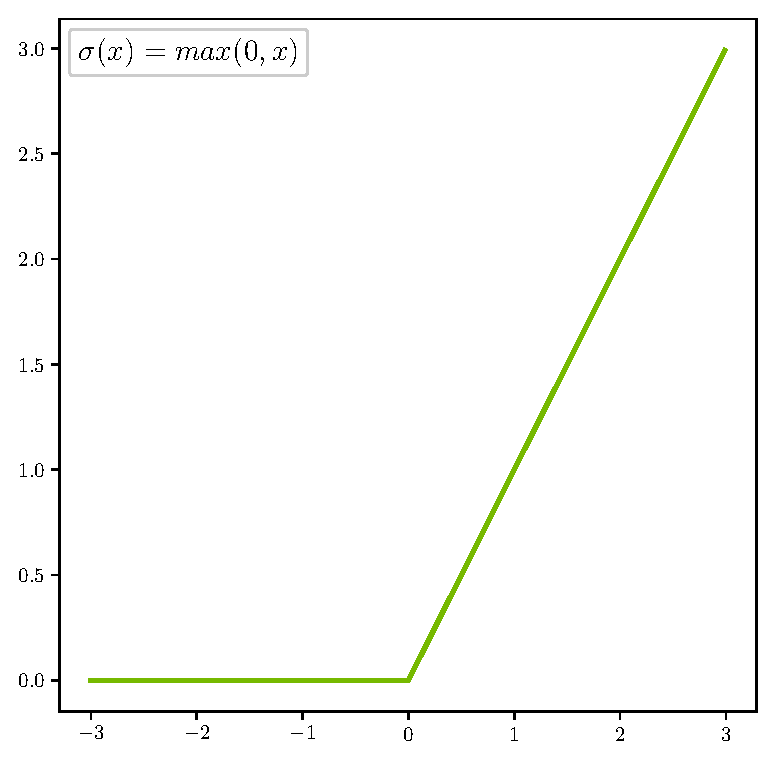
\includegraphics[width=\textwidth]{resources/images/ReLU.eps}
        \caption{ReLU\footnotemark}
        \label{fig:relu}
    \end{subfigure}
    \hfill
    \begin{subfigure}[b]{0.3\textwidth}
        \centering
        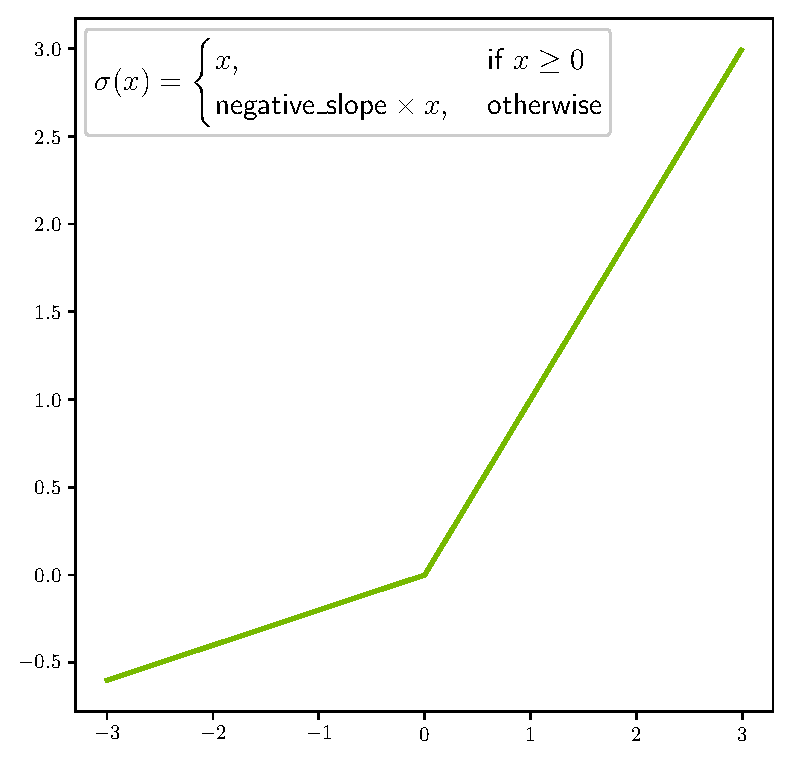
\includegraphics[width=\textwidth]{resources/images/LReLU.eps}
        \caption{LReLU\footnotemark}
        \label{fig:lrelu}
    \end{subfigure}
    \hfill
    \begin{subfigure}[b]{0.3\textwidth}
        \centering
        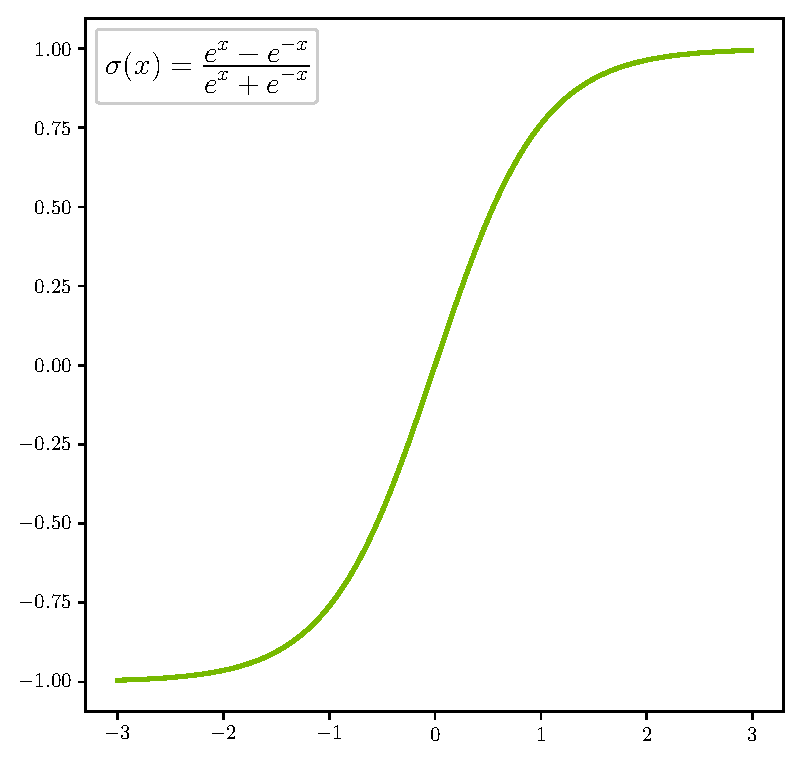
\includegraphics[width=\textwidth]{resources/images/Tanh.eps}
        \caption{Tanh\footnotemark}
        \label{fig:tanh}
    \end{subfigure}
    \caption{The Generator and Discriminator use these 3 activation functions: ReLU, LReLU and Tanh}
    \label{fig:activation_functions}
\end{figure}


\footnotetext[5]{ReLU: \url{https://pytorch.org/docs/stable/generated/torch.nn.ReLU.html}}
\footnotetext[6]{LReLU: \url{https://pytorch.org/docs/stable/generated/torch.nn.LeakyReLU.html}}
\footnotetext[7]{Tanh: \url{https://pytorch.org/docs/stable/generated/torch.nn.Tanh.html}}


\newpage


\subsubsection{Determined AI - Training Loop}

The Determined AI training loop is a simple method of the PyTorchTrial class. Determined AI passes batches from the configured data loader of the configured batch size to this method. The function is responsible for optimizing the neural networks. The user can decide which values he wants to return and make available on the Determined AI dashboard. In the case of this project, the author returns multiple different loss values. \\

\begin{listing}[H]
\inputminted{python}{resources/codes/train_batch.py}
\captionof{lstlisting}{The main training loop method of Determined AI}
\end{listing}

The first step in a WGAN is to optimize the Discriminator. To do that, one needs to sample a  random vector $ z $ from a normal distribution and pass it to the Generator to create fake images. Fake images and actual images pass through the Discriminator and their scores through the loss function and the gradient penalty function, which the author explains in \ref{sec:loss_function} and \ref{sec:gradient_penalty}. The total loss is the sum of the two. Determined AI offers methods to calculate the backward pass and perform the optimization step. Note that in lines 5-6, the Generator gradients are not calculated.  \\

\begin{listing}[H]
\inputminted{python}{resources/codes/optimize_discriminator.py}
\captionof{lstlisting}{How to opimize the Discriminator}
\end{listing}

\newpage

To train the Generator, the Discriminator only needs to calculate the scores of the generated fake images. The scores pass to the Generator's loss function, and the backward function uses it to calculate the gradients. Afterward, the Generator's optimizer performs an optimization step on the Generator's weights.

\begin{listing}[H]
\inputminted{python}{resources/codes/optimize_generator.py}
\captionof{lstlisting}{How to opimize the Generator}
\end{listing}

\subsubsection{Loss Function}
\label{sec:loss_function}

Generator and Discriminator use different loss functions. Both loss functions together form the WGAN loss. Adding the negative mean of the actual images' scores and the positive mean of the fake images' scores calculates the Discriminator loss. The Generator's loss calculates by averaging over the negative scores of the fake images.

\begin{listing}[H]
\inputminted{python}{resources/codes/wgan_loss.py}
\captionof{lstlisting}{Code for the WGAN-Loss}
\end{listing}


\newpage

\subsubsection{Gradient Penalty}
\label{sec:gradient_penalty}

Adding a regularization term to the Discriminator's total loss ensures that the Discriminator satisfies the  Lipschitz-1 constraint.

\begin{listing}[H]
\inputminted{python}{resources/codes/gradient_penalty.py}
\captionof{lstlisting}{Code of the Gradient Penalty}
\end{listing}

Line 1-2 calculate an intermediate image representation by picking a random location on a straight line between real and fake images. These interpolated images pass to the Discriminator in Line 5. Afterward, PyTorch's autograd calculates the Discriminator's gradients. Line 9 forms the Euclidean norm of each tensor in the gradients batch, then subtracts it by one and takes it to the power of two. The final gradient penalty is the mean of the before calculated norms multiplied with a coefficient of 10.

\newpage

\subsection{Evaluation}
\label{sec:evaluation}


The author performs eight different experiments to test the performance and the image quality of the generated images. All experiments use Adam as the optimizer for Discriminator and Generator. The author sets the Discriminators learning rate to $ 0.0004 $ and the Generators learning rate to $ 0.0001 $. This configuration is in the paper \citetitle{heusel2018ttur} \cite{heusel2018ttur}. It proves that it can omit the need for multiple Discriminator updates. \\


\begin{table}[H]
    \ra{1.3}
    \centering
    \begin{tabular}{@{}lllllllll@{}}
    \toprule
    \# & Optimizer & $ lr_{g} $ & $ lr_{d} $ & $ \beta_{g} $ & $ \beta_{d} $ & $ depth_{g} $ & $ depth_{d} $ & $ dim_{z} $ \\ \midrule
    1 & Adam & 0.0001 & 0.0004 & 0.5, 0.999 & 0.5, 0.999 & 8  & 8  & 128 \\
    2 & Adam & 0.0001 & 0.0004 & 0.5, 0.999 & 0.5, 0.999 & 16 & 16 & 128 \\
    3 & Adam & 0.0001 & 0.0004 & 0.5, 0.999 & 0.5, 0.999 & 32 & 32 & 128 \\
    4 & Adam & 0.0001 & 0.0004 & 0.5, 0.999 & 0.5, 0.999 & 64 & 64 & 128 \\ \bottomrule
    \end{tabular}
    \caption{Experiment configurations with the CelebA HQ dataset}
\label{tab:experiments_celeba_hq}
\end{table}

Both optimizers use the same beta values $ \beta_{1} $ and $ \beta_{2} $ of 0.5 and 0.999. All experiments transform the vector $ z $ with a dimension of 128 to 64x64 RGB images. Each experiment varies in the Generators and Discriminator's depth. The depth is a multiplier for the number of filters in the networks. A higher depth means more parameters and, therefore more trainable degree of freedom. The experiments examine the effect of the depth parameter on the generated image quality. \\

\begin{table}[H]
    \ra{1.3}
    \centering
    \begin{tabular}{@{}lllllllll@{}}
    \toprule
    \# & Optimizer & $ lr_{g} $ & $ lr_{d} $ & $ \beta_{g} $ & $ \beta_{d} $ & $ depth_{g} $ & $ depth_{d} $ & $ dim_{z} $ \\ \midrule
    5 & Adam & 0.0001 & 0.0004 & 0.5, 0.999 & 0.5, 0.999 & 8  & 8  & 128 \\
    6 & Adam & 0.0001 & 0.0004 & 0.5, 0.999 & 0.5, 0.999 & 16 & 16 & 128 \\
    7 & Adam & 0.0001 & 0.0004 & 0.5, 0.999 & 0.5, 0.999 & 32 & 32 & 128 \\
    8 & Adam & 0.0001 & 0.0004 & 0.5, 0.999 & 0.5, 0.999 & 64 & 64 & 128 \\ \bottomrule
    \end{tabular}
    \caption{Experiment configurations with the Anime Face dataset}
\label{tab:experiments_anime_face}
\end{table}

\newpage